% One chessboard row: occupied columns 0, 2 and 5 encode 100101_2 = 37.
% The leftmost cell represents the least significant bit.
% Regenerate from this directory with:
% latex -interaction=nonstopmode -halt-on-error state-kings.tex
% dvisvgm --no-fonts --exact --bbox=papersize -o state-kings.svg state-kings.dvi
\documentclass[tikz,border=0pt]{standalone}
\definecolor{darkcell}{HTML}{BC9200}
\definecolor{lightcell}{HTML}{FFE7A0}
\begin{document}
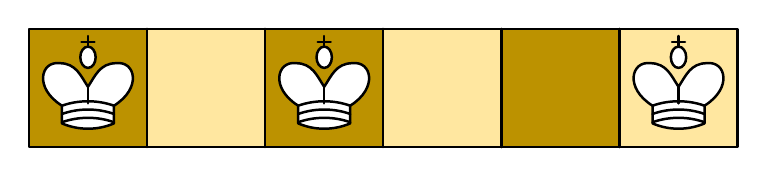
\begin{tikzpicture}[x=1.5cm,y=1.5cm,line width=0.9pt,line cap=round,line join=round]
  \foreach \column in {0,...,5} {
    \pgfmathtruncatemacro{\parity}{mod(\column,2)}
    \ifnum\parity=0
      \fill[darkcell] (\column,0) rectangle (\column+1,1);
    \else
      \fill[lightcell] (\column,0) rectangle (\column+1,1);
    \fi
  }
  \draw (0,0) rectangle (6,1);
  \foreach \column in {1,...,5} \draw (\column,0) -- (\column,1);
  % A self-contained vector king, avoiding a platform-specific chess font.
  \foreach \column in {0,2,5} {
    \begin{scope}[shift={(\column+0.5,0.48)}]
      \draw (0,0.35) -- (0,0.46) (-0.055,0.41) -- (0.055,0.41);
      \draw[fill=white] (0,0.28) ellipse (0.065 and 0.09);
      \draw[fill=white]
        (-0.22,-0.13)
        .. controls (-0.46,0.02) and (-0.4,0.25) .. (-0.24,0.23)
        .. controls (-0.1,0.23) and (-0.06,0.12) .. (0,0.03)
        .. controls (0.06,0.12) and (0.1,0.23) .. (0.24,0.23)
        .. controls (0.4,0.25) and (0.46,0.02) .. (0.22,-0.13)
        -- (0.22,-0.28)
        .. controls (0.08,-0.34) and (-0.08,-0.34) .. (-0.22,-0.28)
        -- cycle;
      \draw (0,0.03) -- (0,-0.11);
      \draw (-0.22,-0.13) .. controls (-0.08,-0.08) and (0.08,-0.08) .. (0.22,-0.13);
      \draw (-0.22,-0.2) .. controls (-0.08,-0.15) and (0.08,-0.15) .. (0.22,-0.2);
      \draw (-0.22,-0.27) .. controls (-0.08,-0.22) and (0.08,-0.22) .. (0.22,-0.27);
    \end{scope}
  }
\end{tikzpicture}
\end{document}
